\documentclass[a4paper, 14pt]{extarticle}
\input{../../.preambles/10-russian}
\input{../../.preambles/20-math}
\usepackage[utf8]{inputenc}
\usepackage[paper=a4paper, top=1cm, right=1cm, bottom=1.5cm, left=2cm]{geometry}
\usepackage{setspace}
\usepackage{ifthen}
\usepackage{array}
\usepackage{bm}
\onehalfspacing

\usepackage{graphicx}
\graphicspath{{plots/}, {images/}}

\parindent=1.25cm

\renewcommand{\thesection}{\arabic{section}.}
\renewcommand{\thesubsection}{\arabic{section}.\arabic{subsection}.}
\numberwithin{equation}{section}

\usepackage{caption}
\DeclareCaptionLabelFormat{figure}{Рисунок #2}
\DeclareCaptionLabelFormat{table}{Таблица #2}
\DeclareCaptionLabelSeparator{sep}{~---~}
\captionsetup{labelsep=sep,justification=centering,font=small}
\captionsetup[figure]{labelformat=figure}
\captionsetup[table]{labelformat=table}

\usepackage{titlesec}
\titleformat{\section}
    {\centering\normalsize\bfseries}
    {\thesection}
    {1em}{}
\titleformat{\subsection}
    {\normalsize\bfseries}
    {\thesubsection}
    {1em}{}

% Настройка вертикальных и горизонтальных отступов
\titlespacing*{\section}{\parindent}{*4}{*4}
\titlespacing*{\subsection}{\parindent}{*4}{*4}

\usepackage[square, numbers, sort&compress]{natbib}
\makeatletter
\bibliographystyle{unsrt}
\renewcommand{\@biblabel}[1]{#1.} 
\makeatother
\addto\captionsrussian{\def\bibname{Список использованных источников}}
\addto\captionsrussian{\def\refname{Список использованных источников}}

\newcolumntype{C}[1]{>{\centering\arraybackslash}m{#1\textwidth}}
\renewcommand{\arraystretch}{1.2}

\usepackage{color}
\definecolor{darkgreen}{rgb}{0,.5,0}
\usepackage[colorlinks,linkcolor=black,filecolor=blue,citecolor=darkgreen,urlcolor=black]{hyperref}

\newcommand{\maketitlepage}[1]{
    \begin{titlepage}
        \singlespacing
        \newpage
        \begin{center}
            Министерство образования и науки Российской Федерации \\
            Федеральное государственное бюджетное образовательное \\
            учреждение высшего профессионального образования \\
            <<Волгоградский государственный технический университет>> \\
            Факультет электроники и вычислительной техники \\
            Кафедра физики
        \end{center}
        \vspace{9em}
        \begin{center}
           { \large\bfseries ОТЧЕТ }
            \\ О научно-исследовательской практике на \( \underset{\text{наименование организации}}{\rule{.35\textwidth}{.5pt}\hrulefill} \)
        \end{center}
        \vspace{4em}
        \begin{table}[h!]
            \center         
            \begin{tabular}{b{.3\textwidth}ccl}
                Руководитель практики от организации & \( \underset{\text{должность}}{\rule{3cm}{.5pt}\hrulefill} \) & \( \underset{\text{подпись}}{\rule{3cm}{.5pt}\hrulefill} \) & Виснер~С.~В. \\
                Руководитель практики от университета & доцент & \( \underset{\text{подпись}}{\rule{3cm}{.5pt}\hrulefill} \) & Поляков~И.~В. \\
                Студент группы Ф-369 & \multicolumn{2}{c}{\( \underset{\text{подпись}}{\rule{6.5cm}{.5pt}\hrulefill} \)} & #1
            \end{tabular}
        \end{table}
        \vspace{5em}

        \begin{flushright}
            \begin{minipage}{.5\textwidth}
                Отчет защищен с оценкой \hrulefill
            \end{minipage}
        \end{flushright}
        \vspace{\fill}
        \begin{center}
            Волгоград, \the\year
        \end{center}

    \end{titlepage}
    \setcounter{page}{2}
}

\input{../../.preambles/10-russian}
\input{../../.preambles/20-math}

\begin{document}
\maketitlepage{Чечеткин~И.~А.}
\setcounter{page}{3}

\section*{Аннотация}

В данной работе приведены цели и задачи научно-исследовательской практики, а также описаны принципы проектирования импульсного источника питания (за основу взятисточник питания на 12 вольт). Приведено краткое описание прохождения практики
(электрическая схема блока питания, описание практической части).

\section*{Список ключевых понятий}

Трансформатор, випер, диодный мост, SMD-монтаж, дроссель, индуктивность,
рассеиваемая мощность, накопительный конденсатор.

\newpage

\tableofcontents
\newpage

\section{Введение}
Прохождение практики студентами на предприятии подразумевает собой ознакомление
студентов с реальным технологическим процессом и закреплением теоретических
знаний, полученных в ходе обучения.
	
На протяжении долгого времени остается актуальным вопрос о производстве
различных источников питания, ведь от них зависит нормальное функционирование
бытовых электроприборов. Каждый год рынок предлагает большое разнообразие
подобной продукции, имеющую различные входные и выходные характеристики,
соответствующие спросу потребителей. К ним относятся источники питания для
мобильных устройств, силовая электроника, различные инверторы напряжения и т.~п.	
На основе изученной литературы и рынка выпускаемой продукции, была проведена
подготовительная работа, связанная с решением поставленной задачи. За основу
блока питания была использована схема обратноходового преобразователя.
	
Преобразователь с передачей энергии на обратном ходу (обратноходовой
преобразователь, \emph{Flyback}, флайбэк) можно назвать одной из самых
популярных топологий импульсных источников питания.

Основное преимущество обратноходовой топологии~-- дешевизна и малое количество
деталей. Поэтому практически все сетевые источники питания до мощностей
30--50~Вт строятся именно по этой топологии. Флайбэк прекрасно справляется с
формированием нескольких выходных напряжений с неплохой стабильностью
дополнительных напряжений, не требуя при этом практически никаких
схемотехнических изысканий.
\newpage

\section{Принцип действия и основные соотношения}
\begin{figure}[h!]
    \center
    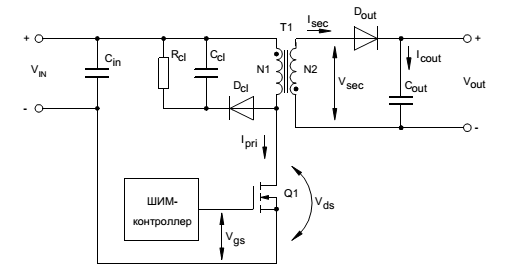
\includegraphics[width=.6\textwidth]{m_01}
\parbox{.6\textwidth}{\caption{Силовая часть обратноходового
преобразователя}\label{p01}}
\end{figure}
На рис.~\ref{p01} изображена силовая часть обратноходового преобразователя, а нарис.~\ref{p02}~-- диаграммы его основных токов и напряжений.
        
\begin{figure}[h!]
    \begin{minipage}{.5\textwidth}
Будем анализировать самый распространенный режим работы~-- режим разрывных токов(\emph{discontinuous}). Это значит, что к началу следующего цикла вся энергия изтрансформатора передана в нагрузку, и следующий цикл начинается с нулевого тока
в
трансформаторе. Режим безразрывных токов (\emph{continuous}) распространен
гораздо меньше.
        
Для анализа разобьем рабочий цикл на отдельные периоды. Пусть схема работает на
частоте \( f \), при этом период будет \( T = 1/f \). Интервал \( t_0 - t_1
\)~-- время включенного состояния силового ключа \( Q_1 \) (время прямого
хода)~-- обозначим как \( t_{ON} \), соответственно рабочий цикл (\emph{Duty
Circle}, в дальнейшем \( D \)) будет определяться как \( D = t_{ON}/T \).
        
\textbf{Интервал \( \bm{t_0 - t_1} \).} К моменту \( t_0 \) сердечник
трансформатора полностью размагничен, и ток в нем отсутствует. В момент, когда сШИМ-контроллера подается управляющий сигнал, силовой
    \end{minipage} \hfill
    \begin{minipage}{.45\textwidth}
        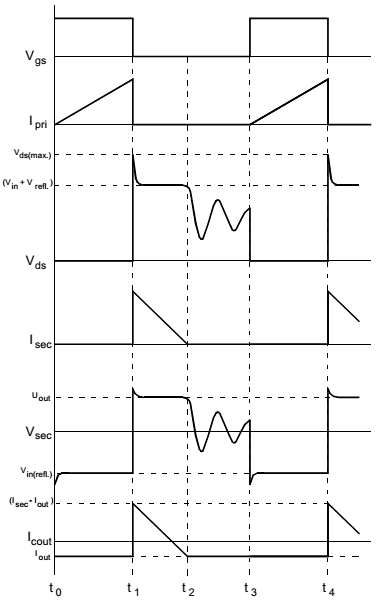
\includegraphics[width=\textwidth]{m_02}
\parbox{\textwidth}{\caption{Диаграммы токов и напряжений обратноходового
преобразователя}\label{p02}}
    \end{minipage}
\end{figure}
\noindent ключ \( Q_1 \) открывается и ток в трансформаторе начинает нарастать.
То есть в идеализированной схеме включение силового транзистора происходит при
нулевом токе. В реальных же условиях происходит некоторый бросок тока, связанныйс зарядом паразитных емкостей трансформатора, что при больших входных
напряжениях приводит к существенным потерям в ключе и возникновению паразитных
высокочастотных колебаний. Для уменьшения последних стремятся несколько
замедлить процесс открывания транзистора для уменьшения паразитных токов.
Выходной диод также полностью закрыт к этому времени, и нет необходимости в
быстром его перезаряде/восстановлении.

Ток в индуктивности первичной обмотки трансформатора \( L_{PRI} \) будет
нарастать до тех пор, пока ШИМ-контроллер не даст команду на выключение силовоготранзистора. ШИМ-контроллер рассчитывает (исходя из сигнала рассогласования
обратной связи) количество энергии, которую необходимо запасти для поддержания
постоянной мощности в нагрузке плюс потери в самом источнике. Если мощность в
нагрузке обозначить как \( P_{OUT} \), то за время прямого хода мы должны
запасти следующее количество энергии:
\begin{equation}
    A = \frac{P_{OUT}}{\eta\cdot f},
\end{equation}
где \( \eta \)~-- коэффициент полезного действия (КПД).

Энергия, запасаемая в индуктивности есть:
\begin{equation}
    A = \frac{L\cdot I_{PRI}^2}{2},
\end{equation}
и можно найти ток, который нарастет в первичной обмотке трансформатора за время
прямого хода:
\begin{equation}
I = \sqrt\frac{2\cdot A}{L_{PRI}} = \sqrt\frac{2\cdot P_{OUT}}{\eta\cdot f\cdot
L_{PRI}}.
\end{equation}
Для определения необходимой индуктивности первичной обмотки будет использоваться
это соотношение совместно с формулой:
\begin{equation}
    U = L\cdot\der{I}{t}.
\end{equation}

Любопытно, что величина импульсного тока не зависит от входного напряжения~--
это позволяет строить прекрасно работающие на практике схемы ограничения
выходного тока (точнее, выходной мощности).

Теперь следует узнать среднеквадратичное значение первичного тока~-- это
необходимо для расчета потерь в силовом ключе и в обмотке трансформатора. Для
тока пилообразной формы среднеквадратичное его значение будет: 
\begin{equation}
    I_{RMS} = I_{PRI}\cdot\sqrt\frac{D}{3}.
\end{equation}
Соответственно, статические потери в силовом ключе будут:
\begin{equation}
    P_{DC} = I_{RMS}^2\cdot R_{DC},
\end{equation}
где \( R_{DC} \) -- сопротивление канала открытого транзистора.

Потери в первичной обмотке в общем случае считаются с учетом эффекта близости.

На вторичной обмотке во время этого интервала ток нагрузки поддерживается
исключительно выходным конденсатором. К выходному диоду \( D_{OUT} \) приложено
трансформированное входное напряжение. Если первичная обмотка содержит \( N_1 \)
витков, а вторичная~-- \( N_2 \), то коэффициент трансформации
\begin{equation}
    K = \frac{N_1}{N_2},
\end{equation}
и обратное напряжение на диоде \( D_{OUT} \) есть:
\begin{equation}
    V_{D_{OUT}} = \frac{V_{IN}}{K} + (V_{OUT} + V_D),
\end{equation}
где \( V_D \)~-- прямое падение напряжения на выходном диоде.

При использовании диодов Шоттки с недостаточным запасом по напряжению в этом
интервале могут возникнуть проблемы~-- при большом напряжении обратный ток диода
Шоттки может достигать существенных значений~-- единиц и даже десятков
миллиампер, что вкупе с большим обратным напряжением создает большую
рассеиваемую мощность, особенно при повышенной температуре~-- здесь можно легко
получить потери превышающие даже потери от протекания прямого тока.

\textbf{Интервал \( \bm{t_1 - t_2} \)}.

Силовой транзистор выключается, ток в нем резко спадает от \( I_{PRI} \) до
нуля, а напряжение начинает быстро расти и достигает \( V_{MAX} \). Можно
ожидать, что в этот момент происходит большое выделение энергии от динамических
потерь. К сожалению, оценить их достаточно сложно, слишком много параметров
влияет на скорость этого процесса, и влияние времени переключения весьма и
весьма высоко. В общем случае:
\begin{equation}
    P_{SW} = \frac{I_{PRI}\cdot V_{MAX}\cdot t_{SW}\cdot f}{2}.
\end{equation}
Интервал время \( t_{SW} \) зависит от энергии переключения силового
транзистора, суммарного сопротивления в цепи его затвора, напряжения питания
выходного каскада драйвера, индуктивности в цепи истока. Но первичный ток также
начинает перезаряжать паразитную емкость трансформатора, снижая скорость
нарастания напряжения на ключе. Этот эффект снижает динамические потери (а
иногда вообще может свести их влияние к нулю). Поэтому влияние динамических
потерь оказывается гораздо более существенным для \emph{DC-DC}~конверторов с их
низкими входными напряжениями, большими первичными токами и высокими частотами
преобразования, а в сетевых источниках становятся существенными потери от
перезаряда паразитной емкости:
\begin{equation}
    P_{SW,\ CAP} = \frac{C_p\cdot V_{SW}^2\cdot f}{2}.
\end{equation}

\section{Заключение}
\newpage

\phantomsection\addcontentsline{toc}{section}{Список литературы}
\begin{thebibliography}{9}
    \bibitem{Koshljakov}Кошляков,~Н.~С. Уравнения в частных производных
    математической физики [Текст] / Кошляков~Н.~С., Глинер~Е.~Б., Смирнов~М.~М.
    Учебное пособие. -- М.: <<Высшая школа>>, 1970.-- 712с.
\end{thebibliography}
\end{document}